\subsection{要求妥当性確認}

要求妥当性確認とは、現在理解されている要求が、利害関係者の真のニーズを表しているかを確認する活動である。英語では \,\en{Requirements Validation}\, と呼ばれる。

ここで大切なのは、「正しく書かれているか」だけではなく、「そもそもこれを作れば問題が解決するか」を見ることである。要求文が文法的に正しくても、利用者の実際の困りごとを解決しないなら妥当ではない。

\MiniBox{妥当性確認で問うこと}{要求はこの時点で必要なものを十分に含んでいるか。不要な要求はないか。理解しやすいか。矛盾していないか。標準や契約に合っているか。}

\subsubsection{要求レビュー}

\term{要求レビュー}{Requirements Review}は、要求文書やモデルを人が読んで確認する方法である。もっとも一般的な妥当性確認手段である。

\term{レビュー}{Review}には複数の視点が必要である。顧客や利用者は、自分たちのニーズが正しく表されているかを見る。要求の専門家は、文書が明確で、標準に沿っているかを見る。設計者や開発者は、設計・実装に必要な情報があるかを見る。テスト担当は、テスト可能かを見る。

\subsubsection{シミュレーションと実行}

形式的またはモデルベースの要求仕様では、仕様を手作業またはツールで\term{実行}{Execution}または\term{シミュレーション}{Simulation}できることがある。利用者は、文章を読むよりも、シナリオに沿って動く様子を見る方が理解しやすい場合がある。

\subsubsection{プロトタイピング}

\term{プロトタイプ}{Prototype}とは、本格的な実装の前に作る試作品である。画面の動き、操作感、処理の流れ、重要な技術的可能性などを具体的に示すために使う。

プロトタイプは、技術者の解釈を利害関係者に見せ、誤解を早く発見するのに有効である。ただし、見た目の細部や一時的な品質問題に関心が向きすぎると、本来確認したい要求から注意がそれることがある。

\par\smallskip
\begin{center}
\centering
\IfFileExists{assets/generated_figures/ch01/fig-ch01-09.png}{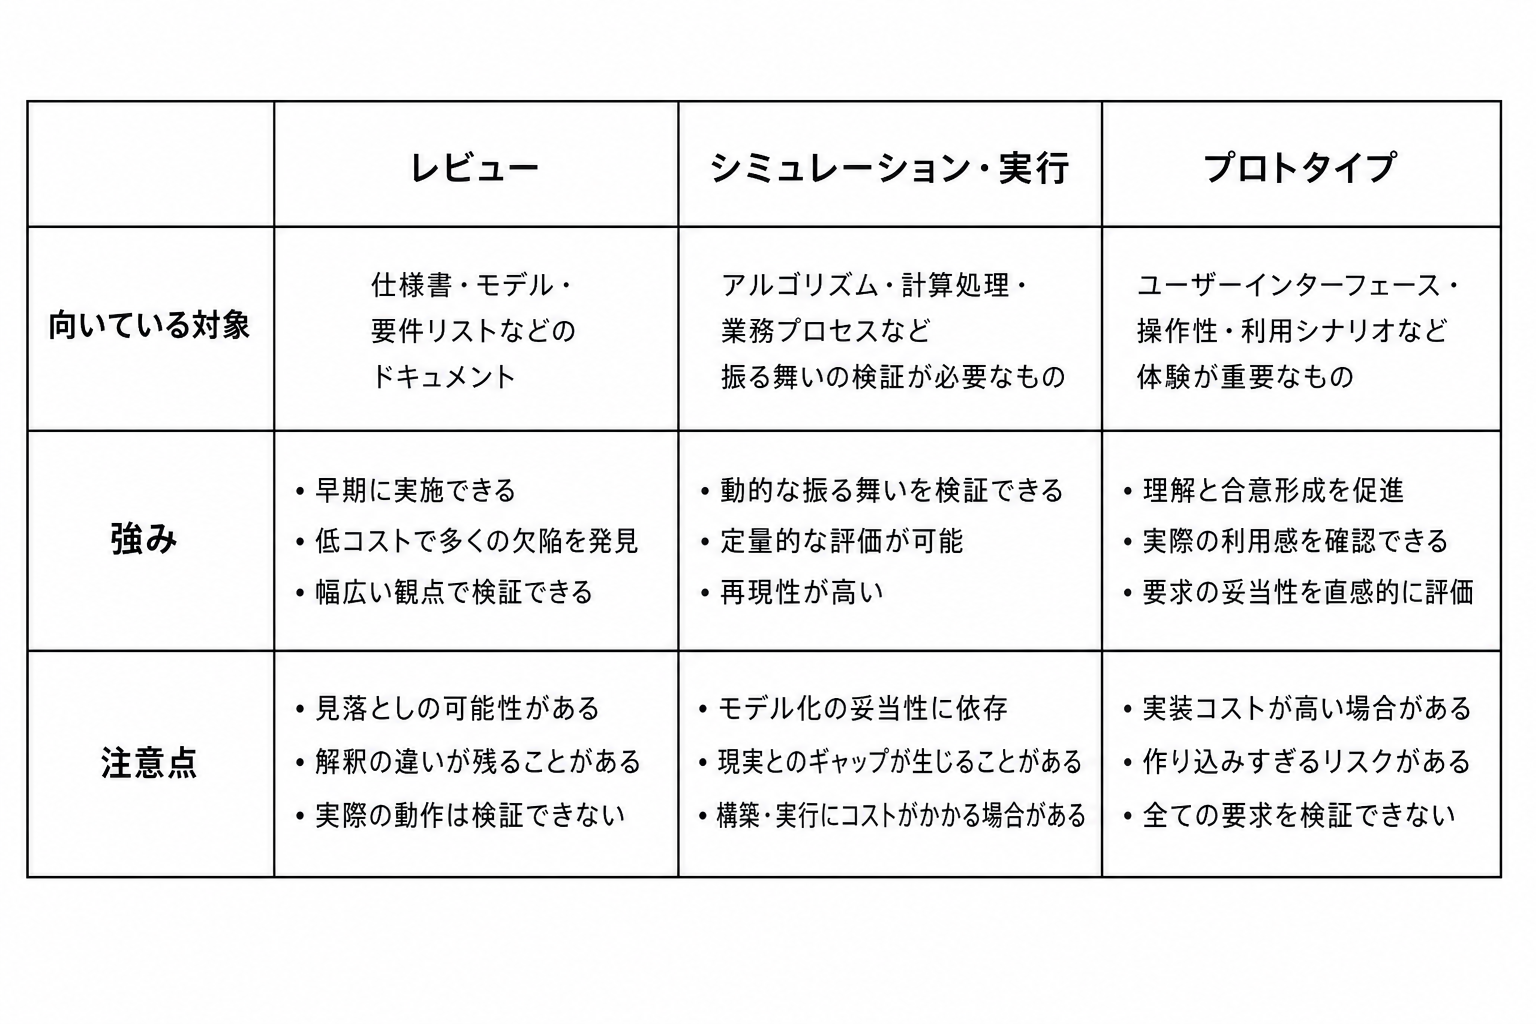
\includegraphics[width=0.96\linewidth]{assets/generated_figures/ch01/fig-ch01-09.png}}{\fbox{\parbox[c][48mm][c]{0.9\linewidth}{\centering 画像生成待ち\\要求妥当性確認の三手法を比較する図}}}
\par\smallskip
\refstepcounter{figure}\label{fig:ch01-09}図 \thefigure: 要求妥当性確認の三手法を比較する図
\end{center}
図 \thefigure は、要求妥当性確認の三手法を比較する図を視覚的に整理したものである。
\par\smallskip
